\documentclass[border=10pt]{standalone}
\usepackage{tikz}
\usetikzlibrary{arrows.meta, positioning, calc, fit}
\usepackage{xcolor}
\usepackage{amsmath, amssymb}

% Brand colors
\definecolor{Garnet}{HTML}{73000A}
\definecolor{Atlantic}{HTML}{466A9F}
\definecolor{Congaree}{HTML}{1F414D}
\definecolor{Horseshoe}{HTML}{65780B}
\definecolor{Rose}{HTML}{CC2E40}
\definecolor{LightGray}{HTML}{ECECEC}
\definecolor{WarmGrey}{HTML}{676156}
\definecolor{Black90}{HTML}{363636}

\begin{document}
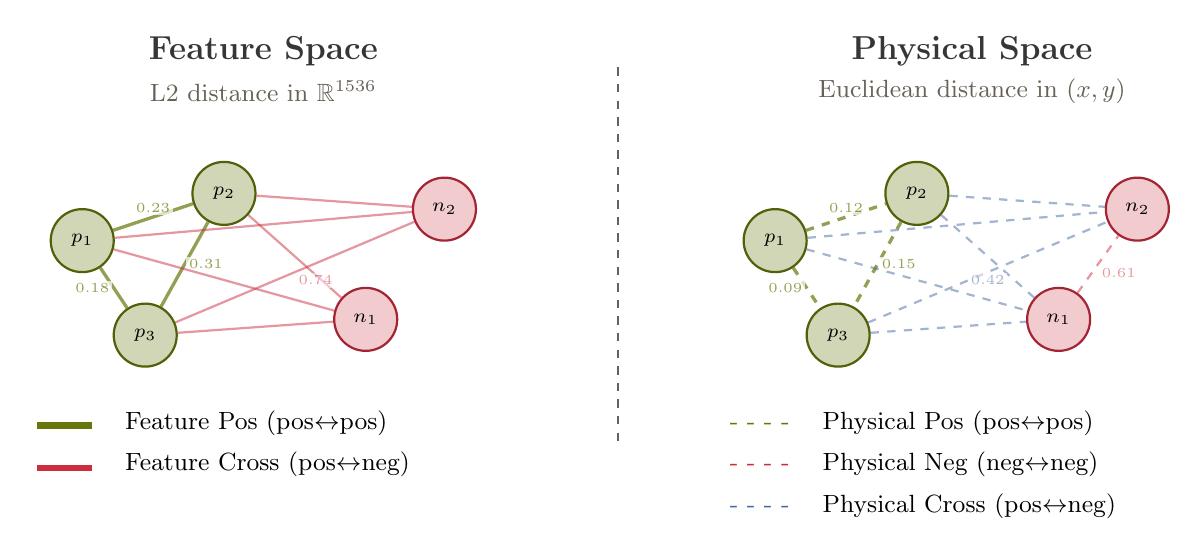
\begin{tikzpicture}[
    posnode/.style={circle, draw=Horseshoe!80!black, fill=Horseshoe!30, thick,
        minimum size=0.8cm, font=\scriptsize\bfseries, inner sep=0pt},
    negnode/.style={circle, draw=Rose!80!black, fill=Rose!25, thick,
        minimum size=0.8cm, font=\scriptsize\bfseries, inner sep=0pt},
    seclbl/.style={font=\large\bfseries, Black90},
    every node/.style={font=\normalsize}
]

% =============================================
% LEFT: Feature Space
% =============================================
\node[seclbl] at (3.5, 7.2) {Feature Space};
\node[font=\small, WarmGrey] at (3.5, 6.7) {L2 distance in $\mathbb{R}^{1536}$};

\node[posnode] (fp1) at (1.2, 4.8) {$p_1$};
\node[posnode] (fp2) at (3.0, 5.4) {$p_2$};
\node[posnode] (fp3) at (2.0, 3.6) {$p_3$};
\node[negnode] (fn1) at (4.8, 3.8) {$n_1$};
\node[negnode] (fn2) at (5.8, 5.2) {$n_2$};

% feature_pos edges
\draw[Horseshoe, very thick, opacity=0.7] (fp1) -- (fp2)
    node[midway, above, font=\tiny, fill=white, inner sep=1pt, text=Horseshoe] {0.23};
\draw[Horseshoe, very thick, opacity=0.7] (fp1) -- (fp3)
    node[midway, left, font=\tiny, fill=white, inner sep=1pt, text=Horseshoe] {0.18};
\draw[Horseshoe, very thick, opacity=0.7] (fp2) -- (fp3)
    node[midway, right, font=\tiny, fill=white, inner sep=1pt, text=Horseshoe] {0.31};

% feature_cross edges
\draw[Rose, thick, opacity=0.5] (fp1) -- (fn1);
\draw[Rose, thick, opacity=0.5] (fp2) -- (fn2);
\draw[Rose, thick, opacity=0.5] (fp3) -- (fn1);
\draw[Rose, thick, opacity=0.5] (fp2) -- (fn1);
\draw[Rose, thick, opacity=0.5] (fp1) -- (fn2);
\draw[Rose, thick, opacity=0.5] (fp3) -- (fn2)
    node[midway, below right, font=\tiny, fill=white, inner sep=1pt, text=Rose] {0.74};

% Legend
\node[font=\small, anchor=north west] at (0.5, 2.8) {
    \begin{tabular}{@{}cl@{}}
    \textcolor{Horseshoe}{\rule{0.7cm}{2.5pt}} & Feature Pos (pos$\leftrightarrow$pos) \\[4pt]
    \textcolor{Rose}{\rule{0.7cm}{2pt}} & Feature Cross (pos$\leftrightarrow$neg) \\
    \end{tabular}
};

% =============================================
% Divider
% =============================================
\draw[WarmGrey, thick, dashed] (8.0, 7.0) -- (8.0, 2.2);

% =============================================
% RIGHT: Physical Space
% =============================================
\node[seclbl] at (12.5, 7.2) {Physical Space};
\node[font=\small, WarmGrey] at (12.5, 6.7) {Euclidean distance in $(x,y)$};

\node[posnode] (pp1) at (10.0, 4.8) {$p_1$};
\node[posnode] (pp2) at (11.8, 5.4) {$p_2$};
\node[posnode] (pp3) at (10.8, 3.6) {$p_3$};
\node[negnode] (pn1) at (13.6, 3.8) {$n_1$};
\node[negnode] (pn2) at (14.6, 5.2) {$n_2$};

% physical_pos edges
\draw[Horseshoe, very thick, dashed, opacity=0.7] (pp1) -- (pp2)
    node[midway, above, font=\tiny, fill=white, inner sep=1pt, text=Horseshoe] {0.12};
\draw[Horseshoe, very thick, dashed, opacity=0.7] (pp1) -- (pp3)
    node[midway, left, font=\tiny, fill=white, inner sep=1pt, text=Horseshoe] {0.09};
\draw[Horseshoe, very thick, dashed, opacity=0.7] (pp2) -- (pp3)
    node[midway, right, font=\tiny, fill=white, inner sep=1pt, text=Horseshoe] {0.15};

% physical_neg edges
\draw[Rose, thick, dashed, opacity=0.5] (pn1) -- (pn2)
    node[midway, below right, font=\tiny, fill=white, inner sep=1pt, text=Rose] {0.61};

% physical_cross edges
\draw[Atlantic, thick, dashed, opacity=0.5] (pp1) -- (pn1);
\draw[Atlantic, thick, dashed, opacity=0.5] (pp2) -- (pn2);
\draw[Atlantic, thick, dashed, opacity=0.5] (pp3) -- (pn1);
\draw[Atlantic, thick, dashed, opacity=0.5] (pp2) -- (pn1);
\draw[Atlantic, thick, dashed, opacity=0.5] (pp1) -- (pn2);
\draw[Atlantic, thick, dashed, opacity=0.5] (pp3) -- (pn2)
    node[midway, below, font=\tiny, fill=white, inner sep=1pt, text=Atlantic] {0.42};

% Legend
\node[font=\small, anchor=north west] at (9.3, 2.8) {
    \begin{tabular}{@{}cl@{}}
    \textcolor{Horseshoe}{- - - -} & Physical Pos (pos$\leftrightarrow$pos) \\[4pt]
    \textcolor{Rose}{- - - -} & Physical Neg (neg$\leftrightarrow$neg) \\[4pt]
    \textcolor{Atlantic}{- - - -} & Physical Cross (pos$\leftrightarrow$neg) \\
    \end{tabular}
};


\end{tikzpicture}
\end{document}
